\documentclass[10pt,a4paper]{article}
\usepackage[utf8]{inputenc}
\usepackage{amsmath, graphicx, varioref, verbatim, geometry}
\usepackage{amsfonts}
\usepackage{amssymb}
\usepackage{hyperref}
\usepackage{caption}
\usepackage{subcaption}
\begin{document}
\title{FYS-STK4155, Autumn 2019, Project 3}
\author{Aksel Kristofer Gravir (akselkg)}
\maketitle

\begin{abstract}
I implement a feed-forward scheme and an analytical solution solving the 1-d heat equation, then show an approach using a dense neutral network also can be used to solve the same equation. Finally this approach is used to try find eigenvalues and vectors of a small symmetric matrix, with unconvincing results.
\end{abstract}


\section*{Part a)}
The problem to solve is the dimensionless one-dimensional heat equation on a bounded interval
\[u_{xx} = u_t, t>0, x \in [0,1],\]
with initial conditions 
\[u(x,0) = \sin(\pi x),\]
and fixed (Dirichlet) boundary conditions
\[u(0,t) = 0, u(1,t) = 0\]

To find an analytic solution we start by assuming we can separate $u$ into a product of functions of only one of the variables $(x,t)$
\[u(x,t) = X(t)T(t).\]
Inserted into the differential equation we get
\[X_{xx}T= XT_t\]
\[\frac{X_{xx}}{X} = \frac{T_t}{T} = k\]
where k is a constant since the individual fractional function expressions are independent in their variables. This means we have two ordinary differential equations
\[X_{xx} - kX = 0,\]
\[T_t - kT = 0.\]
These are relatively simple to solve, using the boundary conditions, but I'll skip the details. We end up with a countably infinite set of solutions 
\[X_n = \sin(n \pi x)\]
\[T_n = B_n \exp(-(n\pi)^2 t),\]
\[u_n = X_n T_n = B_n \sin(n \pi x) \exp(-(n\pi)^2 t)\]
for each $n \geq 1$, where $B_n$ is a constant. Since differentiation is a linear operator linear combinations of these solutions are also solutions. To match the initial condition we need to determine $B_n$ so that
\[\sum_{n=1}^{\infty} u_n(x,0) = u(x, 0).\]
By a simple examination this holds for $B_1 = 1$, all other $B_n = 0$. So 
\[u = sin(\pi x) \exp(-\pi^2 t)\]
is the analytical solution to the equation.

\begin{figure}[!ht]
	
	\begin{center}
		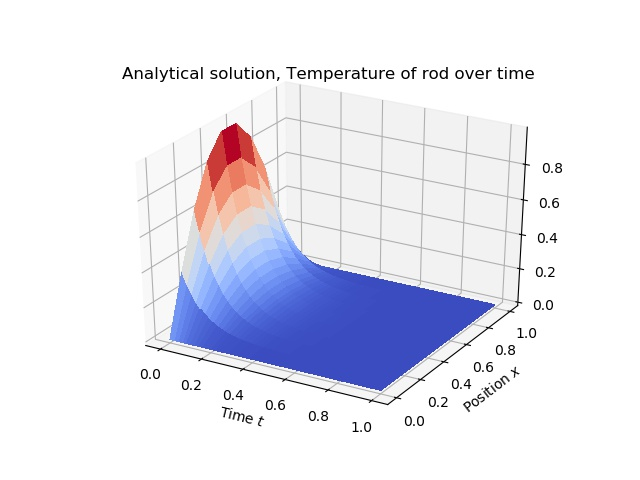
\includegraphics[width=\textwidth]{surface_plot.jpg}
	\end{center}
	\label{surface}
	
\end{figure}

To solve the system numerically we use the explicit forward Euler algorithm with a centered difference in space given by the relationships
\[u_t \approx \frac{u(x,t+\Delta t) - u(x,t)}{\Delta t}\]
\[u_{xx} \approx \frac{u(x + \Delta x,t) - 2u(x,t) + u(x - \Delta x,t)}{\Delta x^2}.\]

Then we discretize these expressions. I will use the shorthand notation $u_i^j= u(x_i, t_j)$. 
\[u_{xx} = u_{t}\]
\[\frac{u_{i+1}^j - 2u_i^j + u_{i-1}^j}{\Delta x^2} = \frac{u_i^{j+1} - u_i^j}{\Delta t}\]
We have one term in $u_i^{j+1}$, which will represent the next time step in our scheme.
\[u_i^{j+1} = \left(1 - 2\frac{\Delta t}{\Delta x^2}\right) u_i^j + \frac{\Delta t}{\Delta x^2} \left(u_{i+1}^j + u_{i-1}^j\right)\]
 Using this expression we can directly calculate each point inside our boundary. 

\section*{Part b)}

The Euler forward scheme is implemented in the function forward\_scheme(u0, t), that returns the end state of the system after time $t$. For meaningful inputs the entire progression of the system over time is not visually distinguishable from the surface plot of $u(x,t)$ in Fig. \ref{surface}. At individual slices in time there are some slight differences for the coarsest of the two suggested $\Delta x$ values, $\frac{1}{10}$. These results are shown in Fig. \ref{slice}. It is not so strange that the scheme seems to work very well, since the geometry and the initial conditions are very simple. The shape of the initial condition represent the shape of least rapid change, since the exponential term in the analytic solution only has a term where $n=1$.

\begin{figure}[!ht]
	
	\begin{center}
		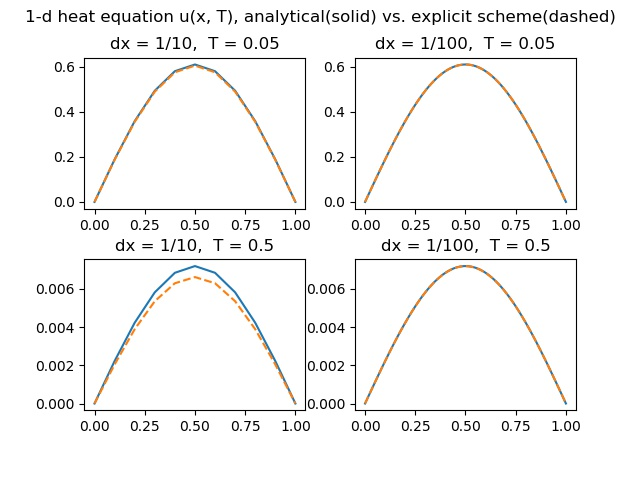
\includegraphics[width=\textwidth]{forward_plot.jpg}
	\end{center}
	\label{slice}
	
\end{figure}

\section*{Part c)}

I implemented a dense neural network using Tensorflow, following the lecture notes discussing how to implement solutions to differential equations using machine learning. As a trial function I used
\[(1-t)*u(x) + x*(1-x)*t*\text{dnn\_output}.\]
The extra terms in $x$ and $t$ are there to ensure that the boundary and initial conditions are true. 
The cost function used was 
\[MSE(0, u_t - u_{xx}),\]
this term enforces the differential equation on the network. One example run of the network using two hidden layers of 90 and 10 nodes with 100000 iterations yielded the result shown in Fig. \ref{nnplot}
\begin{figure}[!ht]
	
	\begin{center}
		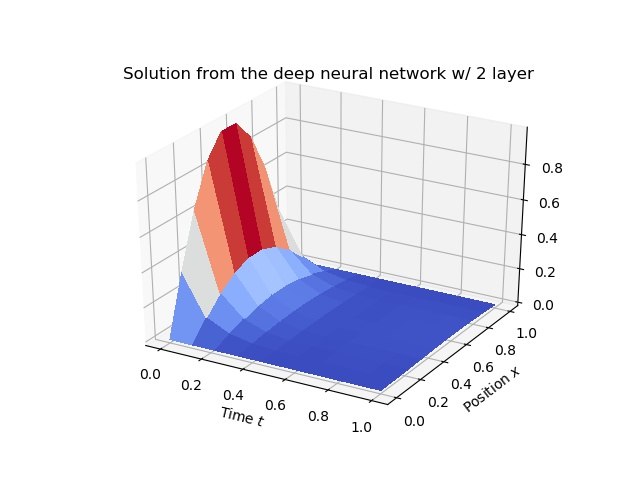
\includegraphics[width=\textwidth]{nn_plot.jpg}
	\end{center}
	\label{nnplot}
	
\end{figure}

My program additionally output:
\begin{verbatim}
Max absolute difference between analytical solution and TensorFlow DNN =  0.01858410023266266
Mean square error between analytical solution and TensorFlow DNN =  1.6375012482184538e-05
\end{verbatim}

Some additional plots of slices of the same set-up are in Fig. \ref{nnslice}

\begin{figure}[!ht]
	
	\begin{center}
		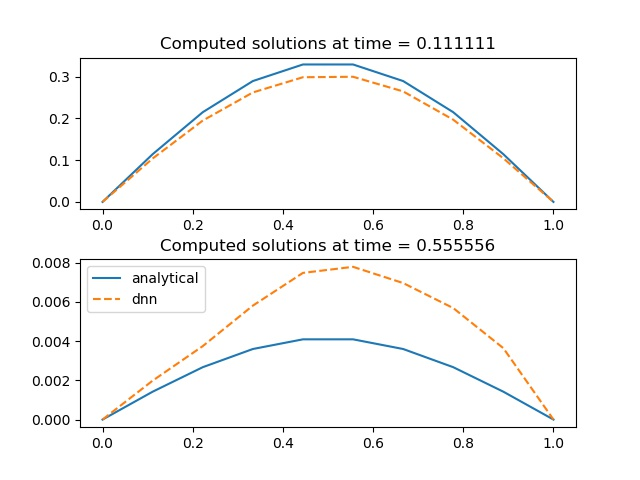
\includegraphics[width=\textwidth]{slices_nn_plot.jpg}
	\end{center}
	\title*{Slices of result running the network using two hidden layers of 90 and 10 nodes with 100000 iterations.}
	\label{nnslice}
	
\end{figure}

\section*{Part 4)}
By modifying the differential equation solver further I did implement a solver for finding eigenvectors/values. However my results were quite poor for any input I tested. With a $5\times 5$ symmetric matrix, 10000 iterations and ten points in time, I found the eigenvector
\begin{verbatim}
[-0.45310531 -0.60174178 -0.14652591  0.11431227  0.57977958]
\end{verbatim}

from a matrix with eigenvectors

\begin{verbatim}
array([[-0.61279592,  0.44521535, -0.455395  ,  0.45316052,  0.1162987 ],
       [ 0.678675  ,  0.46974298,  0.02325843,  0.52952073, -0.19444438],
       [ 0.39153705, -0.14763236, -0.83388728, -0.23373013,  0.27368897],
       [-0.09906257,  0.08820331, -0.28418448, -0.2727824 , -0.909525  ],
       [-0.0276902 , -0.74266391, -0.126276  ,  0.62065556, -0.21569565]].
\end{verbatim}

Which does not seem to match! It seems pointless to use this calculate the corresponding eigenvalue. The cost function seems to converge to a stable value over time. If i had to guess i would say the error is in the expression of the cost function, or possibly in the function $f(x)$, which was quite complex to calculate.

\section*{e)}

\end{document}